\subsection{Opdracht 01}

\paragraph{
Geef van een film, de hele reeks waar die bij hoort met volgnummer en in de juiste volgorde.
Indien hij niet in een reeks zit, is de lijst gewoon ��n lang met volgnummer 1.
Dit moet ��n statement worden die van een variabel ID de reeks geeft zoals onderstaand voorbeeld:
DECLARE @MovieInReeks INT = 207989;
}

\begin{lstlisting}
-- jouw statement hier levert onderstaand resultaat:

ITEM_ID		TITLE				Volgnummer
207992		Matrix, The				1
207989		Matrix Reloaded, The			2
207991		Matrix Revolutions, The		3
\end{lstlisting}

\paragraph{

}
\lstinputlisting[language=SQL]{sql/nick/opdracht-01.sql}

\lstinputlisting[language=SQL]{sql/marc/opdracht-01.sql}
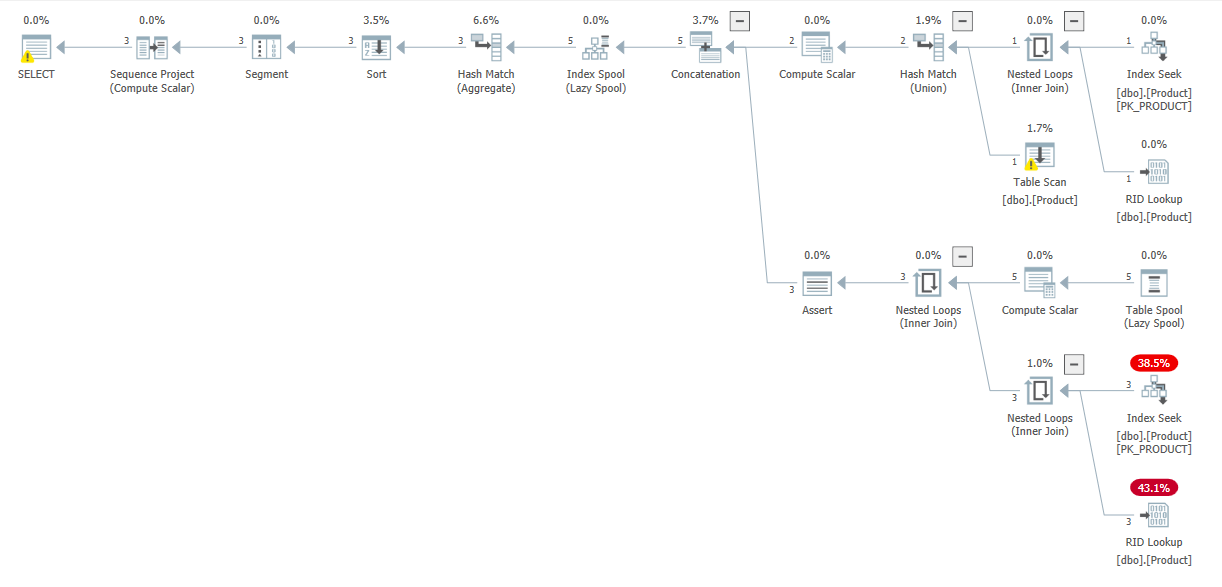
\includegraphics[width=1\textwidth]{image/marc/opdracht-01.PNG}

\lstinputlisting[language=SQL]{sql/joey/opdracht-01.sql}
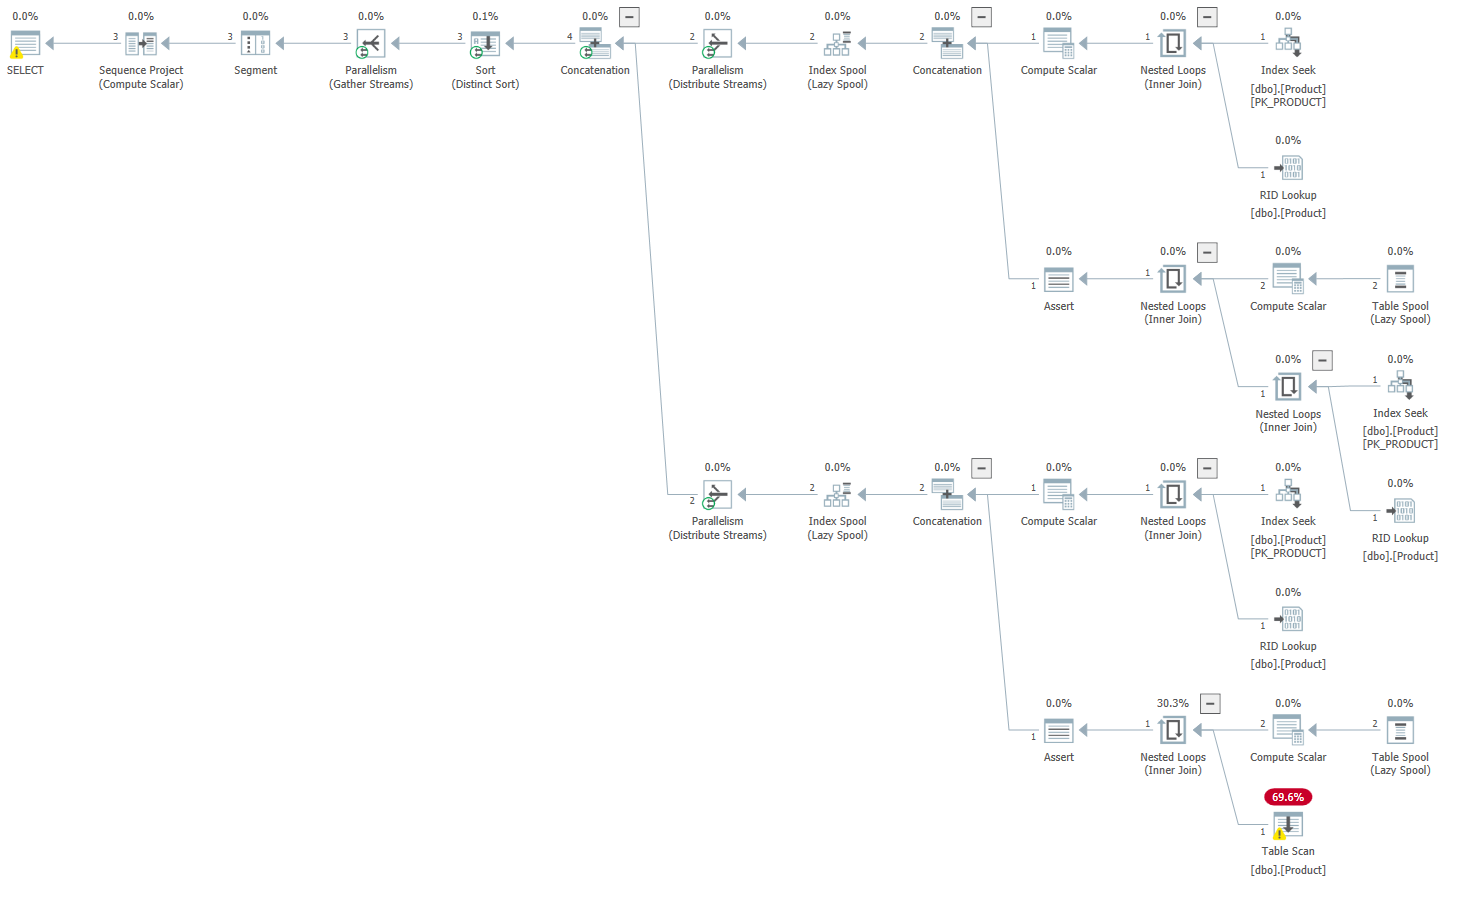
\includegraphics[width=1\textwidth]{image/joey/opdracht-01.PNG}

\paragraph{

}